\documentclass{article}
\usepackage{etex}
%\usepackage[7pt]{moresize}
%\fontfamily{<familyname>}\selectfont
\renewcommand{\sfdefault}{phv}
\usepackage{anyfontsize}
\usepackage{textcomp}
\usepackage{multirow}
\usepackage{standalone}
\usepackage{verbatim}
\usepackage{authblk}
\usepackage{graphicx}
\usepackage{graphics}
\usepackage{multicol}
\usepackage{indentfirst}
\usepackage{pstricks,pstricks-add,pst-math,pst-xkey}
\usepackage{amssymb,amsmath}
\usepackage{algorithm}
\usepackage[noend]{algpseudocode}
\usepackage{float}
\usepackage{filecontents}
\usepackage{flexisym} %% prime symbol
%Lettres francaises
\usepackage[cyr]{aeguill}
\usepackage[francais]{babel}
\usepackage[T1]{fontenc}    %% permet d'utiliser les caractères accentués
\usepackage[utf8]{inputenc} %% permet d'utiliser les caractères accentué
\usepackage{gensymb}
%Needed for problems with bibtex
\usepackage{hyperref}
%PGF plot
\usepackage{pgfplots,pgfplotstable}
\usepgfplotslibrary{statistics}
\pgfplotscreateplotcyclelist{mycolorlist}{blue,red,brown,teal,violet,cyan,green,scarletred1,black}
\pgfplotscreateplotcyclelist{mylegend}{Ly-a,Target,LRG,ELG,Fake,Fake,SS,SF}
\usepackage{xifthen}

\usepackage{tikz}
\usepgfplotslibrary{external}
\usetikzlibrary{pgfplots.external} 
\usetikzlibrary{shapes,shadows,arrows}
%\tikzexternalize[prefix=figs/graph/]% activate with a name prefix
\pgfplotsset{
  compat=newest,
  invoke before crossref tikzpicture={\tikzexternaldisable},
  invoke after crossref tikzpicture={\tikzexternalenable},
}
%\tikzset{external/force next}
%Debug box warnings
\showboxdepth=\maxdimen
\showboxbreadth=\maxdimen
%%%% debut macro %%%%
\newenvironment{changemargin}[2]{\begin{list}{}{%
\setlength{\topsep}{0pt}%
\setlength{\leftmargin}{0pt}%
\setlength{\rightmargin}{0pt}%
\setlength{\listparindent}{\parindent}%
\setlength{\itemindent}{\parindent}%
\setlength{\parsep}{0pt plus 1pt}%
\addtolength{\leftmargin}{#1}%
\addtolength{\rightmargin}{#2}%
}\item }{\end{list}}

\newcommand{\fact}[1]{#1\mathpunct{}!}

%\begin{changemargin}{0cm}{0cm}
%\end{changemargin}

%%%% fin macro %%%%

%Bilio
\usepackage[nottoc,notlof,notlot]{tocbibind}
%Dash lines
\newcommand\Algphasee[1]{%
\Statex\hspace*{-\algorithmicindent}\textbf{#1}%
\vspace*{-.7\baselineskip}\Statex\hspace*{\dimexpr-\algorithmicindent-2pt\relax}\rule{\linewidth}{0.4pt}%
}

\newcommand\Algphase[1]{%
\vspace*{-.7\baselineskip}\Statex\hspace*{\dimexpr-\algorithmicindent-2pt\relax}\rule{\linewidth}{0.4pt}%
\Statex\hspace*{-\algorithmicindent}\textbf{#1}%
\vspace*{-.7\baselineskip}\Statex\hspace*{\dimexpr-\algorithmicindent-2pt\relax}\rule{\linewidth}{0.4pt}%
}

\makeatletter
\def\BState{\State\hskip-\ALG@thistlm}
\makeatother

\def\begeq{\begin{equation}}
\def\endeq{\end{equation}}
\def\begeqar{\begin{eqnarray}}
\def\endeqar{\end{eqnarray}}
\def\Rmm{R_{\rm mm}}
\def\Rdeg{R_{\rm deg}}
\def\micron{\mu{\rm m}}
\def\lya{Ly-$\alpha$\ }
\def\sqd{$deg^{2}$}
\def\psqd{$obj \cdot deg^{-2}$}

\usepackage{geometry}
\geometry{hscale=0.85,vscale=0.85,centering}
\title{Description of fiber assignment code for Mocks in DESI experiment}
%\author{Robert Cahn and Louis Garrigue}
\author[1]{Robert N. Cahn\thanks{rncahn@lbl.gov}}
\author[2]{Louis Garrigue\thanks{louis.garrigue@ens.fr}}
\affil[1]{Department of Cosmological Physics, LBNL, Berkeley}
\affil[2]{Departement de physique, Ecole normale superieure, Paris}
\date{\today}
%--------------------------------------------------------------------------------------------
\begin{document}
\begin{titlepage}
\maketitle
\begin{center}
  \includegraphics[scale=0.2]{python/representant.jpg}

  
\includegraphics[width = 20mm]{figs/logolbnl.png} \hfill
  \includegraphics[width = 20mm]{figs/logodesi.jpg} \hfill
  
\includegraphics[width = 20mm]{figs/logoens.png} 
\end{center}
\end{titlepage}


\section{Introduction}
Martin White started to develop a C++ code for fiber assignment, modified by Lado Samushia, then by Bob Cahn and finally by Bob and Louis Garrigue, intern for 5 months. We included the improvement, redistribution and update steps, to increase the number and the quality of the assignment, and at the same time to have a realistic process, in a way the code can be used. It provides a library of functions which can be easily adapted, with a main producing the assignment. It is well "pipelined" and someone can use it easily. The code can be found on \href{https://github.com/desihub/fiberassign}{DESI git repository} with a short description of how to run it.
  
\section{In a nutshell}
\subsection{Input files}
They are found in the NERSC repository (see features.txt for addresses).
The produced executable (to compile with {\tt make all in src repository)} is {\tt assign}. The calling sequence will look like :
{\tt./assign features.txt}. An example of how runing it on NERSC is provided in the {\tt run} script, then call it with {\tt qsub run}.
 
\begin{itemize} 
	\item Parameters : all parameters used in the fiber assignment are written in this file, including addresses of other input files
	\item Target DB : information, before the study, on all possible targets : (NERSC rep) /projects/projectdirs/desi/mocks/preliminary/objects\_ss\_sf0.rdzipn, created by {\tt make\_catalog}. The samples are taken from Martin's mocks and stored on NERSC at /project/projectdirs/desi/mocks/preliminary/. From these files we create a single file containing the appropriate mix of ELG, LRG, QSO, SS (Standard Stars) and SF (Sky Fibers) using the python script in git fiberassign/bin/make\_catalog\_starsandsky.py. In the same place there is python code to produce a mixture of galaxies without any correlations, but with the correct dn/dz
	\item Obs DB : database constructed from the ongoing DESI observations after the data has been processed by the Spectroscopic pipeline. This DB has not been designed yet
	\item Survey tiles : file containing the positions of all the tiles to be observed in /project/projectdirs/desi/software/edison/desimodel/0.3.1/data/footprint/desi-tiles.par
	\item Fiber positions : locations of the positioners in the focal plane in /project/projectdirs/desi/software/edison/desimodel/0.3.1/data/focalplane/fiberpos.txt
\end{itemize} 

To change the location of other input files, one can simply change it in the features file.

\subsection{Output files}
They are produced in a directory defined in features.txt, in the format {\tt tile54.fits} for example for the 54th tile. There are therefore 10666 such binary files. They consist in 5000 lines (fibers) with the following columns :

\begin{itemize}
    \item fiber: [0-4999]
    \item positioner: [0-4999] (not provided yet)
    \item number of available objects
    \item ID of available objects
    \item objtype: ELG, LRG, QSO, SKY, STDSTAR, GAL, OTHER (actually QSOLy-a, or QSOFake etc for now) (-1 if the fiber isn't assigned)
    \item targetid: unique target identifier to get back to target selection info
    \item desi target0: 64 bit mask of targeting info (not yet)
    \item ra: degrees [0-360]
    \item dec: degrees [-90 - +90]
    \item xfocal: mm from center in positioner coordinate system
    \item yfocal: mm from center in positioner coordinate system 
\end{itemize}

\section{Source files}
Source files are file.h and file.cpp and are in this increasing dependency order :
\begin{itemize}
	\item misc : a home-made library of structures (and functions on them) needed to manipulate concerned data, but independent of them. There are pair (of int), List (of int), Table, Cube, and timing, printing, string conversion, error report items.
	\item collision : used to compute collision checking and build polygons representing positioners
	\item features : carries all useful parameters
	\item structs : structures of the manipulated data and their members
	\item global : main high-level functions and algorithms used in the program to collect information, assign fibers, print statistics and output. Important ones are described further
	\item main : neat and quickly understandable code that sums up all the steps of the assignment
\end{itemize}

\section{Parameters}
Here are some features on input galaxies simulated catalog :

\begin{table}[H]\centering
	\begin{tabular}{rcccl} \hline
		Kind&Id&Priority&Nobs&Density (\psqd)\\ \hline
		QSO Ly-$\alpha$ & 0 & 1 & 5 & 50\\
		QSO Tracer & 1 & 1 & 1 & 120\\
		LRG & 2 & 3 & 2 & 300\\
		ELG & 3 & 4 & 1 & 2400\\
		Fake QSO & 4 & 1 & 1 & 90\\
		Fake LRG & 5 & 3 & 1 & 50\\
		Standard Star & 6 & 5 & 1 & 140\\
		Sky Fiber & 7 & 6 & 1 & 1400\\ \hline
	\end{tabular}
	\caption{Characteristics of galaxy samples as set in make\_catalog\_rnc.py}\label{table:characteristics}
\end{table}
A number of parameters are defined in features.txt.
\begin{itemize}
	\item input and output directories
	\item Output = true, whether you want to release the output

	\item Randomize = false randomize order of plates in making plans
	\item Pacman = false selects only spectrometers 0, 1, 2, 7, 8, 9 of the pacman
	\item Npass = 5 number of passes
	\item MaxSS = 10 ; MaxSF = 40 number of fibers assigned to SS and SF on a petal
	\item PlateRadius = $1.65^{\circ}$ radius of the plate
	\item InterPlate = 0 minimal number of plates between two observations of the same galaxy
	\item Analysis = 0, tile distance for getting the information from previously observed tiles
	\item InfDens = false, simulate infinite density of SS and SF

	\item TotalArea = 15789.0 \sqd total area of the sky considered
	\item invFibArea = 700 inverse of area in \sqd accessible to a fiber (fiber density for a \sqd)
	\item moduloGal = 1, if 2 for instance, reads only one object over two in galFile
	\item moduloFiber = 1, same for fiber

	\item PatrolRad = 6.0 mm maximum distance, on plate coordinates, that allows a fiber to a galaxy


	\item Collision = true when we want to allow collisions, to compute the collision rate for instance, and very practical when one wants to make quick tests, to run the fiber assignment faster
	\item Exact = true whether we want exact collision checking (exact geometry of components) or just circles
	\item AvCollide = 3.2 mm in case of no exact collision checking, limit distance between two galaxies for their positioners to collide (so that we have the same collision rate than with exact geometry)
	\item Collide = 1.98 mm minimum distance allowed on plate projection of two assigned galaxies on the same fiber (optimizes collision checking)
	\item NoCollide = 7 mm maximum distance between two galaxies for the collision of their corresponding galaxies (optimizes collision checking)
	\item NeighborRad = 14.0 mm maximum distance to consider that two fibers are neighbors

	\item PlotObsTime, etc, whether we want to plot some information into output files
	\item Verif = false, whether we verificate that the assignment is sane (no collision, sane mapping, etc...)
\end{itemize}


\section{Classes and structures}
Classes and structures are built to be independent of each other, flexible, quickly understandable, logical, and with no redundant information as much as possible.

\begin{table}[H]\begin{center}
	\begin{tabular}{|l|l|p{11cm}|} \hline
		Structure name & Meaning & Description \\ \hline \hline

		element & Element of a geometric figure & Either a set of juxtaposed segments, either a circle\\ 

		polygon & Polygon of segments + circles & Set of elements\\ \hline

		Feat & Features/Parameters & Carries all needed parameters defined in features.txt and some other computed in the input reading process\\ \hline

		PP & Plate Parameters & Carries locations of positioners on the plate, spectrometer correspondence, and neighboring fibers information\\ 

		onplate & Plate coordinates & Used for coordinates in the focal plane in mm\\ 

		plate & A plate & Locations in the sky of the tile in terms of a unitary vector derived from RA and DEC. Carries also the Id of the tile, its pass, and the available galaxies it is able to reach. Plates is vector of plate, and carries all information on tiles\\ \hline

		galaxy & A galaxy & Information on a galaxy : kind which corresponds to Table \ref{table:characteristics}, a position in the sky (in two differents ways), and the available tile-fibers that can observe it. Gals is vector of galaxy and carries all information on galaxies\\ \hline

		Assignment & An entire assignment & Carries mapping of tile-fibers to galaxies on a table, and other redundant information for optimization\\ \hline
	\end{tabular}\end{center}
	\caption{Classes and structures}\label{tab:structures}
\end{table}


\section{Functions}
In algorithms, j stands for a plate, k for a fiber, p for a petal, g for a galaxy. They are integers in the code.

\subsection{Improvement functions ideas}
Here we present the three ideas of improvement of this first assignment, which increase the number of used fibers and the quality of the assignment. It represents the body, the main purpose of our work. They need to be somewhere "orthogonal", so that they don't loose efficiency when we call one of them after an other.
Those three ideas are coded into the three following functions :

\begin{center}\rule{8cm}{0.4pt}\end{center}

\begin{figure}[H]
	\hspace*{5cm}
	\includegraphics[scale=1]{figs/graph/idea.pdf}
	\hspace*{1cm}
	\includegraphics[scale=1]{figs/graph/transf.pdf}\hfill
	\caption{Improve}\label{transf}
\end{figure}

The idea is to take an unassigned fiber and to look at the galaxies it can reach and that are already assigned. We then look at the second fiber, which is observing this galaxy and try to reassign it to an other galaxy, and assign the first fiber to the first object. It is powerful because we use it when making a plan, and so the two fibers can (and are almost always) from different plates, which can be arbitrarily separated.

\begin{center}\rule{8cm}{0.4pt}\end{center}

\begin{figure}[H]
	\hspace*{5cm}
	\includegraphics[scale=1]{figs/graph/idea1.pdf}
	\hspace*{1cm}
	\includegraphics[scale=1]{figs/graph/transf1.pdf}\hfill
	\caption{Redistribute}\label{transf1}
\end{figure}

In redistribute, we look at an assigned fiber, and try to make the observed object observed by and other fiber, which can come from a different plate. It "anneals" the assignment. In this way, it doesn't improves anything, but we then apply the improve function again, which is more efficient. The idea is the improve, then redistribute, then improve again, redistribute etc. If there is no redistribution between a new improve, the improve is almost useless. Furthermore, among possible fibers, we assign it to the least used petal.

\begin{center}\rule{8cm}{0.4pt}\end{center}

\begin{figure}[H]
	\hspace*{5cm}
	\includegraphics[scale=1]{figs/graph/idea2.pdf}
	\hspace*{1cm}
	\includegraphics[scale=1]{figs/graph/transf2.pdf}\hfill
	\caption{Improve from kind}\label{transf2}
\end{figure}

The third idea is to take an assigned fiber that is able to reach a SF (or SS), to assign it, and then we reassign a fiber assigned to a SF. As the number of SF per petal has to remain the same as previously (40) we search the second fiber among the same petal of the first fiber. It's not used anymore since it becomes useless when we first use new\_assign.


\subsection{Some inportant functions in structs.cpp}
{\tt plate\_dist} turns radians into mm on the focal plane, i.e. it is the plate scale as a function of angle.

{\tt projection} combines a galaxy and a particular plate to give the coordinates the galaxy will have in the focal plane when observed as with this tile. It's a rotation in angular coordinates

{\tt find\_collision} returns the fiber number of a fiber that conflicts with tiblefiber (j,k), or -1 if there is no collision 

\subsection{Collecting}
{\tt collect\_galaxies\_for\_all} is multithreaded, and for each fiber of each tile, collects reachable galaxies. It uses kdTree and htmTree libraries written by Martin White. It's absolutely necessary in order to do computations in a reasonable time with supercomputers

{\tt collect\_available\_tilefibers} computes, using the previous work, available tile-fibers for each galaxy (inverse map)

\subsection{Useful sub-functions for global functions}

{\tt ok\_assign\_g\_to\_jk(g,j,k)} checks to see if we can assign g to the tile-fiber (j,k), according to some assigning rules described further (g has to be a QSO, LRG or ELG, only ELG in last pass, and no collision with neighbors)

{\tt find\_best(j,k)} finds the best reachable galaxy for this fiber, according to assignment rules (not observed in two tiles separated by less than Interplate, choose the one with the higher priority, then if several ones compete, the least observed)

{\tt assign\_fiber(j,k)} tries to assign this fiber using find\_best

{\tt improve\_fiber(j0,n,j,k)} if this fiber is unused, tries first to simply assign it, and if it doesn't work, tries to reassign some used one (jp,kp) where $j0\le jp \le j0+n$. Before : (jp,kp) - g ; (j,k) \& gp free. After : (j,k) - g \& (jp,kp) - gp. The power of this function lies in the fact that j and jp can correspond to different passes. Among all galaxies of same priority and same number of observation, it takes the one belonging to the most unused petal, to distribute ELGs

\begin{algorithm}[H]
	\caption{Improve\_fiber(j0,n,j,k)}\label{euclid}
	\begin{algorithmic}[1]
		\If {k is not assigned}
		\State try to assign running assign\_fiber(j,k)
		\If {k couldn't be assigned this way}
		\State initialize a set of variables jp, kp, g, gp
		\For {each galaxy g available to (j,k)}
		\If {it's possible to assign g with k}
		\For {each chosen tile-fibers (jp,kp) which chose g (where $j0\le jp \le j0+n$)}
		\State $gp \leftarrow find\_best(jp,kp)$
		\State memorize jp, kp, g, gp if it's a better set (gp is more worthy) than previous one
		\EndFor
		\EndIf
		\EndFor
		\If {$gp \ne -1$}
		\State Unassign $(jp,kp) \longleftrightarrow g$
		\State Assign $(j,k) \longleftrightarrow g$
		\State Assign $(jp,kp) \longleftrightarrow gp$
		\EndIf
		\EndIf
		\EndIf
	\end{algorithmic}
\end{algorithm}


\subsection{Assigning making a plan}
In the simulated catalog, we know all information on objects (if a QSO is a real one for example). During the real study, one won't have access to this information prior to the observation plus analysis time. Thus, in the code, we have to simulate that we have this information only when we have at least once observed the object, and when the analysis of received data tells which exact type it is (fake or not for ELG for example). Algorithms do a plan with only types of objects (QSO, LRG, ELG) available in the catalog. A plan consists of an assignment on a set of consecutive tiles (from 0 to 2000 for instance). The assignment works better when we do only one plan.

The argument "next" (integer) in following functions means that we treat all next "next" plates in the plan we make. If it is $-1$, it will deal with all left plates. For example, if $next\_plate = 10$ and one launch a function with $next = 100$, this function is going to do his job on plates from 10 to 110.

{\tt simple\_assign} makes a first simple assignment plan : for each fiber assign to the best available galaxy

\begin{algorithm}[H]
	\caption{Simple\_assign(j0,n)}\label{euclid}
	\begin{algorithmic}[1]
		\For {each plate j from j0 to j0+n}
		\For {each fiber k in a random order}
		\State try to assign\_fiber(j,k)
		\EndFor
		\EndFor
	\end{algorithmic}
\end{algorithm}

{\tt new\_assign} makes a first assignment plan trying to assign first QSO, then LRG then ELG (neither SS nor SF). This way, a QSO can't be lost because of a collision, among other things.

\begin{algorithm}[H]
	\caption{New\_assign\_fibers(j0,n)}\label{euclid}
	\begin{algorithmic}[1]
		\For {each plate j from j0 to j0+n}
		\For {each petal p of this plate, in a random order}
		\For {each fiber k of this petal, in a random order}
		\State Try assign\_fiber(j,k) only allowing QSO
		\EndFor
		\For {each fiber k of this petal, in a random order}
		\State Try assign\_fiber(j,k) only allowing LRG
		\EndFor
		\For {each fiber k of this petal, in a random order}
		\State Try assign\_fiber(j,k) only allowing ELG
		\EndFor
		\EndFor
		\EndFor
	\end{algorithmic}
\end{algorithm}

{\tt improve} improves the plan applying improve\_fiber to all of the fibers involved in the plan

{\tt improve\_from\_kind (kind)} for every concerned petal, tries to assign unassigned fibers to objects of kind "kind" (useful when it's SS or SF), to release an other fiber (formerly assigned to a SS or SF) that would be reassigned to a regular galaxy (kind is SS or SF when we call it). There is also the function {\tt improve\_fiber\_from\_kind} that does the same but on only a fiber. We don't use it anymore, since we use new\_assign, which already includes potential improvement brought by this function.

\begin{algorithm}[H]
	\caption{Improve\_from\_kind (kind,j0,n)}\label{euclid}
	\begin{algorithmic}[1]
		\For {each plate j from j0 to j0+n}
		\For {each petal p of this plate, in a random order}
		\For {each unassigned fiber k}
		\State initialize a set of variables kp, g, gp
		\For {each available galaxies g of k}
		\For {each fiber kp of p assigned to a galaxy of kind}
		\If {no conflict \& g is worthier than previous one}
		\State memorize kp, g, gp
		\EndIf
		\EndFor
		\EndFor
		\If {$g \ne -1$}
		\State Reassign kp to g
		\State Assign k to a galaxy gp of kind kind
		\EndIf
		\EndFor
		\EndFor
		\EndFor
	\end{algorithmic}
\end{algorithm}

{\tt redistribute\_tf} "anneals" the distribution (so that improve is more efficient after) and in the same time redistribute in a way that the number of unused fibers per petal tends to be the same for every petal. It is very important to prepare the step of assigning SS and SF, in order to replace the least number of ELG and LRG for having the needed number of SS/SF

\begin{algorithm}[H]
	\caption{redistribute\_tf(j0,n)}\label{redis}
	\begin{algorithmic}[1]
		\For {each plate j from j0 to j0+n}
		\For {each assigned fiber k}
		\State get g, the galaxy to which (j,k) is assigned
		\State initialize a set of variables (jpb,kpb) to memorize values of (jp,kp)
		\For {each available tile-fibers of g}
		\If {(jp,kp) is better ($j0\le jp \l j0+n$, unassigned, it's ok to assign, and the petal of (jp,kp) is more unused than the one of (jpb,kpb)) }
		\State memorize (jp,kp) in (jpb,kpb)
		\EndIf
		\EndFor
		\If {$jpb \ne -1$}
		\State Reassign g to (jpb,kpb)
		\EndIf
		\EndFor
		\EndFor
	\end{algorithmic}
\end{algorithm}


{\tt update\_plan\_from\_one\_obs(j)} updates the plan formerly made so that if for example on the plate $j-Analysis$ plates (to simulate there is a delay between observation and result on analysis) we observed a QSO which the analysis reveals fake but is still planed to be observed again further in the plan, we will unassign the corresponding fiber and try to reassign it with improve\_fiber.
In the input catalog we only know the basic type (QSO, LRG, ELG, SS, SF) of the galaxies. The precise type is only infered by a simulation coded in python, but is generated with randomness. So in the algorithms, we can know the nature of the object only when it has been observed once at least and analysed (this delay of "Analysis" number of plates is inserted between those two events). In a plan, we try to optimize assignment, but of course, we can't know the precise type (fake, ...) so it is possible to foresee observing for example 4 times a fake QSO. We won't do it, so after having planned, when we begin to apply it and do the real observation, if we have just previously observed a fake QSO, we will remove further observations in this plan. We then try to assign the released tile-fibers.

\begin{algorithm}[H]
	\caption{Update\_plan\_from\_one\_observation(j0,end\_plan)}\label{euclid}
	\begin{algorithmic}[1]
		\State get the list of galaxies observed by this plate that are discovered fake or target
		\For {each of those galaxies g}
		\State get the list of tile-fibers that are supposed to observed this galaxy further in the plan $j0\le jp \le end_plan$
		\For {each of those tile-fibers (jp,kp)}
		\State Unassign $(jp,kp) \longleftrightarrow g$
		\State run improve\_fiber(j0+1,end-j0,jp,kp) (tries to reassign (jp,kp)
		\EndFor
		\EndFor
	\end{algorithmic}
\end{algorithm}

{\tt assign\_sf\_ss(j)} just before the observation of a tile, we assign SF and SS, replacing ELG then LRG if necessary

\begin{algorithm}[H]
	\caption{assign\_sf\_ss}\label{assignsfss}
	\begin{algorithmic}[1]
		\For {each petal p of this plate, in a random order}
		\State try to assign unused fibers to 40 SF and 10 SS
		\If {not enough SS and/or SF}
		\State try to replace some ELG for SS
		\State try to replace some ELG for SF
		\EndIf
		\If {not enough SS and SF}
		\State try to replace some LRG for SS
		\State try to replace some LRG for SF
		\EndIf
		\EndFor
	\end{algorithmic}
\end{algorithm}

{\tt assign\_left(j)} just before the observation of a tile, for all unassigned fibers, tries to assign them to a galaxy in reach that is supposed to be observed later, and remove the later observation. The goal is to observe and thus analyse objects as soon as possible, not waiting further in the plan.


\subsection{Displaying results}
Histograms are written in Tikz format.

{\tt results\_on\_inputs} displays some statistics on input files (histogram of number of objects in range of a fiber, histogram of number of tile-fibers which can observe a given object, histogram of redshifts by type)

{\tt display\_results} provides the tex-formated results to make Table \ref{res} and writes histograms one can see further in this document

{\tt write\_FAtile\_ascii(j)} writes output of the assignment in ASCII format

{\tt fa\_write(j)} writes output of the assignment in FITS format

{\tt pyplotTile(j)} writes a file tileX.py from which (executing {\tt python tileX.py} one can produce the pdf graphic colored plot of the tile. In it, are also ploted objects requiring more observations. A LRG already observed twice won't appear for example

\section{Rules of assignment}
\begin{itemize}
	\item a tile-fiber is only assigned once
	\item no collision between fiber positioners
	\item two observations of a QSO or an LRG can't be separated by less than {\tt InterPlate} plates
	\item in last pass, only ELG, SS and SF are considered
	\item there are 10 and 40 fibers assigned to SS and SF per petal
	\item basically, we choose best galaxy from at the same time available, observed less than maxgoal(kind) times and unassigned ones. Among them, we take those with highest priority, and then the one which has been seen the least number of times
	\item between an already observed \lya and an unknown QSO, one chooses the already observed \lya
	\item the same SS or SF can be observed several times
	\item SS has priority over SF
	\item our policy is : while improving the assignment, never unassign an object without reassigning it right then
\end{itemize}

\section{Algorithm}
 {\tt main} proceeds by : 
 
 \begin{itemize}
	 \item loading input files : features of galaxies to make F, reading in the galaxies catalog to make G, the positions of the fibers on the plate to make pp, the plate centers and positioner locations to make P
	 \item collect available galaxies for each fiber for each plate, and compute the inverse map (available fibers for each galaxies, useful for improvement functions)
	 \item before begining the study, make a plan of assignment
	 \item begin the study, and update the plan as we get information from objects, ongoing
 \end{itemize}

\subsection{Redistribution-Improvement step}
Assigning only QSO, LRG and ELG, not SS and SF when making the plan leads to have a lot more degrees of freedom for the improvement function, which is then much more efficient. Redistributing unused fibers by petal permits to replace the least ELG possible when assigning SS and SF just before an observation.

When applying the plan, sometimes redistributing-improving the plan is very efficient, it updates the further plan (compared to the initial maked plan, just before begining the study), taking into account that some new fibers have been released and that we have new information on precise kind of objects.
We also do improvement/redistribution process during the observation 5-years time.

Here is presented, in the Figure \ref{unusedfibs0}, histograms of unused fibers per petal, during redistribution/improvement process when making the first plan. The goal is to have 50 unused fibers per petal before begining observations.

\begin{figure}[H]\begin{center}
	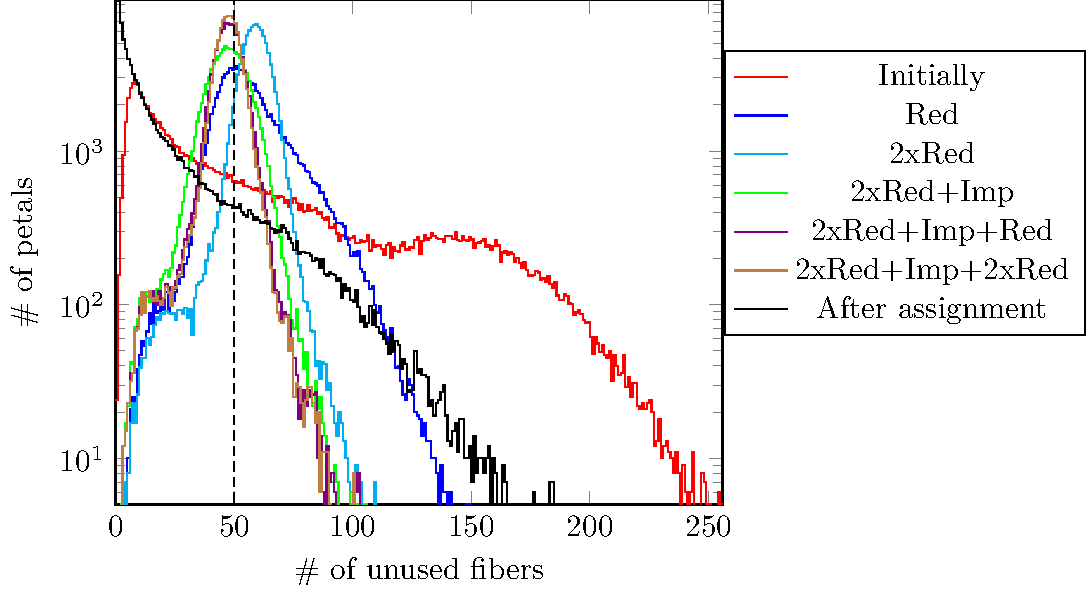
\includegraphics[scale=1]{figs/graph/unusedfibs0.pdf}
	\caption{Unused fibers, at different steps}\label{unusedfibs0}
\end{center}\end{figure}

Here is the the same type of graphic but with more redistributions-improvements, and the same with a linear y axis.

\begin{figure}[H]\begin{center}
	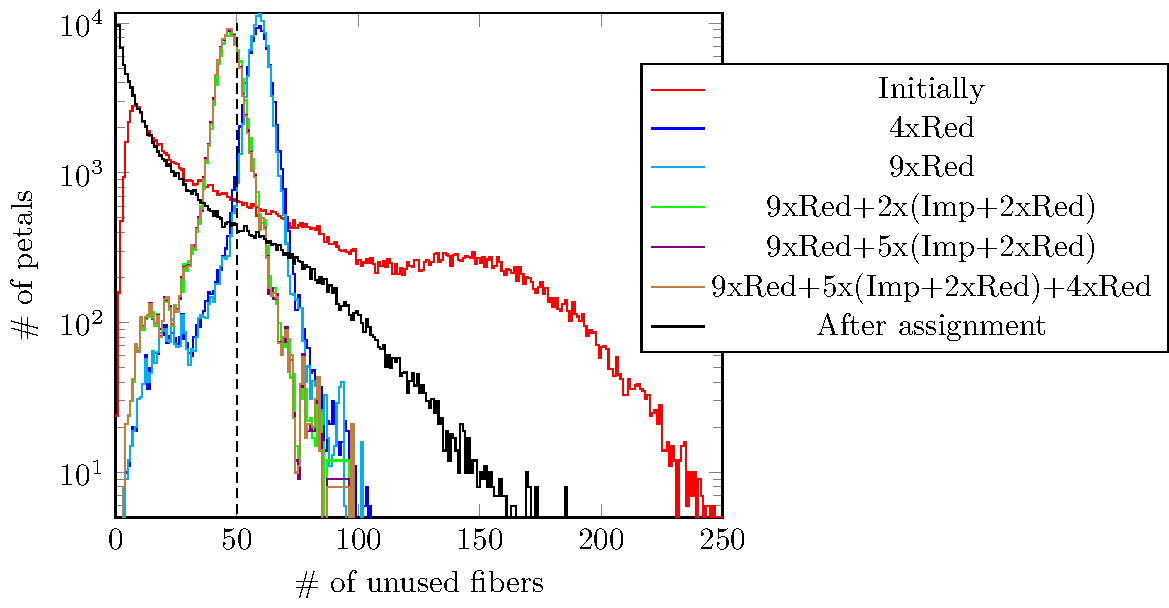
\includegraphics[scale=0.6]{figs/graph/unusedfibs.pdf}
	\caption{Unused fibers, at different steps, with more improvements}\label{unusedfibs}
\end{center}\end{figure}

\begin{figure}[H]\begin{center}
	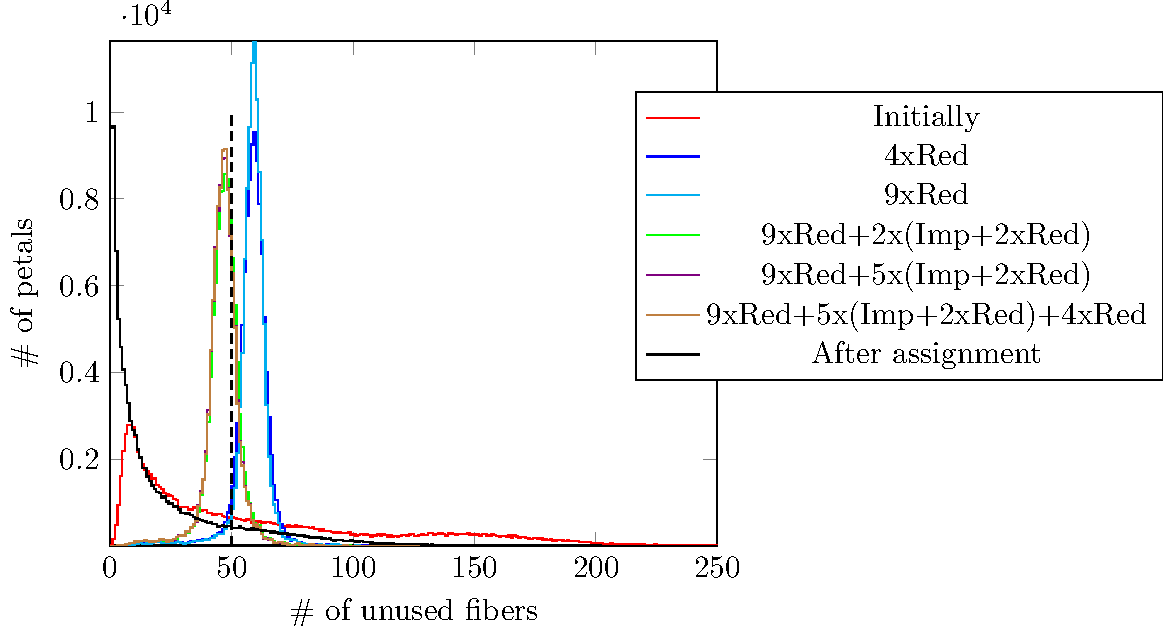
\includegraphics[scale=0.6]{figs/graph/unusedfibsnolog.pdf}
	\caption{Same, no in log scale}\label{unusedfibsnolog}
\end{center}\end{figure}


\subsection{Algorithm, more precisely}

\begin{algorithm}[H]
	\caption{Assignment of reference in main program}\label{euclid}
	\begin{algorithmic}[1]
		\Algphasee{Phase I - Make a plan for all plates}
		\State Run, globally, on the list plates from 0 to last :
		\State "New" assign fibers
		\State Redistribute (several times)
		\State Improve + 2x Redistribute (several times)
		\State Redistribute (several times)
	\end{algorithmic}
	\begin{algorithmic}[1]
		\Algphase{Phase II - Observation time}
		\State Begining of the study
		\For {each plate j of the plan, in order}
		\State Assign\_sf\_ss
		\State Assign\_left
		\State Possibly "pyplot" the planned observed tile
		\State Real observation is here
		\State Update information collected on the previously observed Analysis'th past tile with update\_plan\_from\_one\_obs
		\State If we are in the plate 100, or 300, or 800, or... 2xRedistribute + Improve + Redistribute (on all the plan of remaining tiles)
		\EndFor
	\end{algorithmic}
\end{algorithm}

A standard output display of an execution looks like that (for assignment plan and applying):

{\tt \small 

\noindent\# Read 71,998,144 galaxies from /project/projectdirs/desi/mocks/preliminary/objects\_ss\_sf0.rdzipn \\
\# Read 10,666 plate centers from /project/projectdirs/desi/software/edison/desimodel/0.3.1/data/footprint/desi-tiles.par and 
5000 fibers from /project/projectdirs/desi/software/edison/desimodel/0.3.1/data/focalplane/fiberpos.txt \\
\# Start building HTM tree at 13.8 s \\
\# ... took : 25.5 s \\
\# Begin collecting available galaxies \\
 \# ... took : 31.6 s \\
\# Begin computing available tilefibers \\
\# ... took : 1 mn 12.5 s \\
\# Start assignment at :  2 mn 27 s \\
\# Begin new assignment : \\
  50,518,743 assignments on all left next plates \\
\# ... took : 18 mn 38.3 s \\
\# Begin improve : \\
  565,801 more assignments (1.120 \% improvement) \\
\# ... took : 36.5 s \\
\# Begin redistribute TF : \\
  1,760,465 redistributions of couples of TF \\
\# ... took : 23.3 s \\
\# Begin improve : \\
  206,948 more assignments (0.405 \% improvement) \\
\# ... took : 30.2 s \\
\# Begin redistribute TF : \\
  1,575,337 redistributions of couples of TF \\
\# ... took : 23.1 s \\
\# Begin improve : \\
  92,508 more assignments (0.180 \% improvement) \\
\# ... took : 26 s \\
\# Begin real time assignment at 23 mn 24.5 s \\
 - Plate 0 :   550 not as -  3852 unas \& 2772 replaced \\
 - Plate 1 :    98 not as -  3784 unas \& 2773 replaced \\
 - Plate 2 :   104 not as -  3985 unas \& 2844 replaced \\
 - Plate 3 :   121 not as -  3602 unas \& 2563 replaced \\
 - Plate 4 :   105 not as -  3773 unas \& 2685 replaced \\
 - Plate 5 :    85 not as -  3797 unas \& 2853 replaced \\
 - Plate 6 :   145 not as -  3537 unas \& 2514 replaced \\
 - Plate 7 :    92 not as -  3964 unas \& 2856 replaced \\
 - Plate 8 :   123 not as -  3714 unas \& 2578 replaced \\
- Plate 9 :   143 not as -  3543 unas \& 2378 replaced \\
- Plate 10 :   148 not as -  3528 unas \& 2472 replaced \\
- Plate 11 :    86 not as -  3507 unas \& 2885 replaced \\
\# Begin redistribute TF : \\
  1,160,465 redistributions of couples of TF \\
\# ... took : 23.3 s \\
\# Begin improve : \\
  106,948 more assignments (0.205 \% improvement) \\
\# ... took : 30.2 s \\
- Plate 12 :   48 not as -  3128 unas \& 2475 replaced \\
- Plate 13 :    96 not as -  3407 unas \& 2485 replaced \\
...\\
}

After an observed tile, we print the number of unassigned fibers on it, the number of further objects unassigned because they were analysed as fake, and the number of the corresponding tile-fibers that have been successfully reassigned.

\section{Results}
\subsection{Results on the input catalog}
Here are some statistics on the input galaxies catalog :

\begin{figure}[H]\begin{center}
	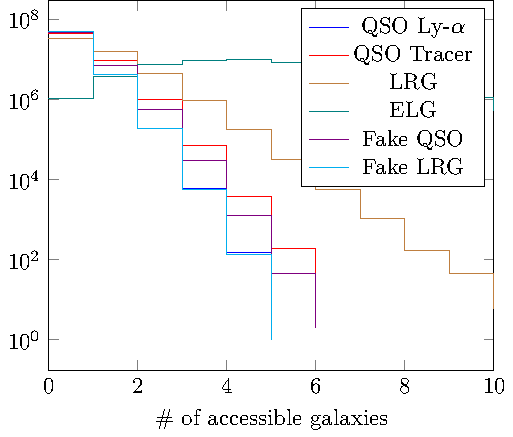
\includegraphics[scale=1]{figs/graph/avgalhist.pdf}
	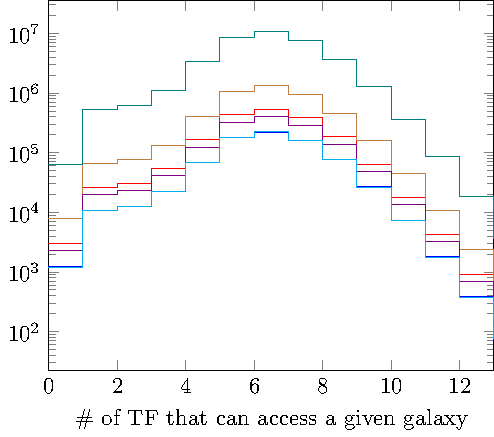
\includegraphics[scale=1]{figs/graph/avtfhist.pdf}\hfill
	\caption{Available galaxies for a fiber on a tile and available tile-fibers for a galaxy (by kind)}\label{avtfhist}
\end{center}\end{figure}

\begin{figure}[H]\begin{center}
	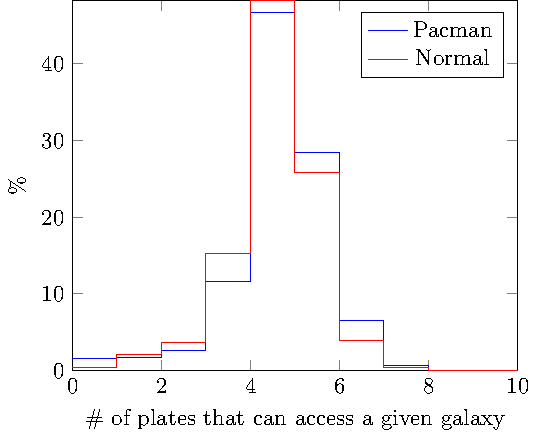
\includegraphics[scale=1]{figs/graph/reachplate.pdf}
	\caption{Available plates for a galaxy (without 5th pass)}\label{reachplate}
\end{center}\end{figure}

\begin{figure}[H]\begin{center}
	\includegraphics[scale=1]{figs/graph/redshifts.pdf}
	\caption{Distribution of objects as a function of redshift}\label{redshifts}
\end{center}\end{figure}

\subsection{Results of the assignment}
We run the program with all information (prior knowledge of information on fake, target, etc) to compare with realistic simulation, this result is interesting to see the effect of this prior unrealistic knowledge.

We have taken a reference strategy, which was a trade-off between computation time and quality of results. We use improvement functions in a way such that they are still efficient given the time they take (because the more improvement execution we launch, the less they are efficient). And from this reference strategy, we change parameters to see the effects of them on the program.

We tried to run it with an "ideal" infinite density of SS and SF, which only led to an 0.5\% inscreasing of the number of observed ELG.

\subsection{Sum-up of assigned galaxies}
The weighted score of a certain kind is defined as : 
\vspace{1\baselineskip}
$Score(kind) = 100\cdot \frac{\sum\limits_{g \in kind} obs(g)}{\sum\limits_{g \in kind} goal}$ where $obs(g)$ is the number of times g is observed.

A sum-up table of general results on assignment is provided on Table \ref{res}.

\begin{table}[H]\begin{center}
\begin{tabular}{rrrrrrrrrrcc}
\hline
\multicolumn{6}{r}{Times observed} \\
	~ &           0 &     1 &  2 & 3 & 4 & 5 &  Total & Fiber used & Once observed & observed $\%$ & weighted $\%$ \\ \hline
    QSOLy-a   &     0 &     1 &   5 & 12 & 19 & 10 &    49 &   180 &    49 & 99.151 & 72.206 \\ 
  QSOTracer   &     1 &   118 &   0 &  0 &  0 &  0 &   119 &   118 &   118 & 99.141 & 99.141 \\ 
        LRG   &    13 &    42 & 243 &  0 &  0 &  0 &   298 &   528 &   285 & 95.505 & 88.434 \\ 
        ELG   &   480 & 1,930 &   0 &  0 &  0 &  0 & 2,411 & 1,930 & 1,930 & 80.054 & 80.054 \\ 
    FakeQSO   &     0 &    89 &   0 &  0 &  0 &  0 &    90 &    89 &    89 & 99.139 & 99.139 \\ 
    FakeLRG   &     2 &    47 &   0 &  0 &  0 &  0 &    50 &    47 &    47 & 95.792 & 95.792 \\ 
\hline
\end{tabular}
\caption{Densities (objects/\sqd) as as a function of \# of observations (with total), and \% observed, once and weighted}\label{res}
\end{center}\end{table}

Furthermore, there are 51,044,452 assignments in total (95.7143 \% of all fibers).

%To be computed !
%\subsection{Pacman plate}
%On the Table \ref{pac}, we present results of the assignment taking for input the fiber locations files of the pacman (plate deprived of 4 petals) used in case of run out of money. Every parameter is the same.

%\begin{table}[H]\begin{center}
%\begin{tabular}{rrrrrrrrrrcc}
%\hline
%\multicolumn{6}{r}{Times observed} \\
	%~ &           0 &     1 &  2 & 3 & 4 & 5 &  Total & Fiber used & Once observed & observed $\%$ & weighted $\%$ \\ \hline


%\hline
%\end{tabular}
%\caption{Same than Table \ref{res} but with the pacman}\label{pac}
%\end{center}\end{table}


\subsection{Free fibers}
Here are the histogram of petals as a function of free fibers and the number of free fibers for each plate, in inscreasing order on Figure \ref{fft}. One can see on the second one the 5 different passes.

\begin{figure}[H]\begin{center}
	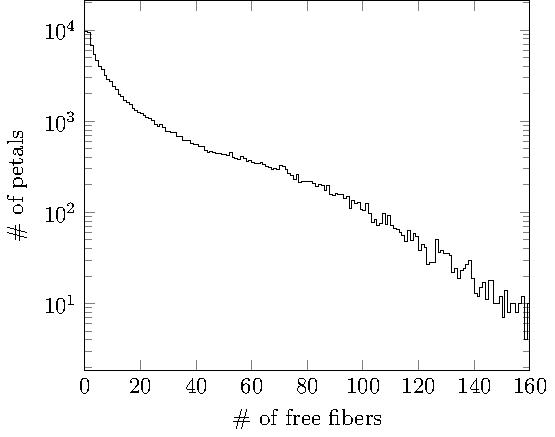
\includegraphics[scale=0.9]{figs/graph/freefib.pdf}
	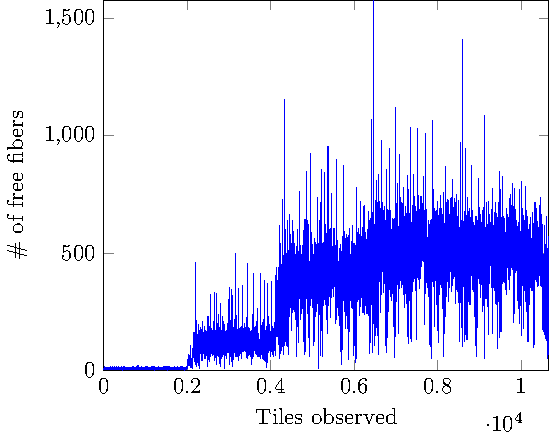
\includegraphics[scale=0.9]{figs/graph/fft.pdf}\hfill
	\caption{\# of petals with that many free fibers and free fibers as a function of time (plates)}\label{fft}
\end{center}\end{figure}

On Figure \ref{seendens}, one can see the proportion of observed objects as a function of their density. "usq" stands for unity of square degrees, it's the area of the sky reachable by a single fiber. As expected, when density inscreases, proportion of observed objects decreases.

\begin{figure}[H]\begin{center}
	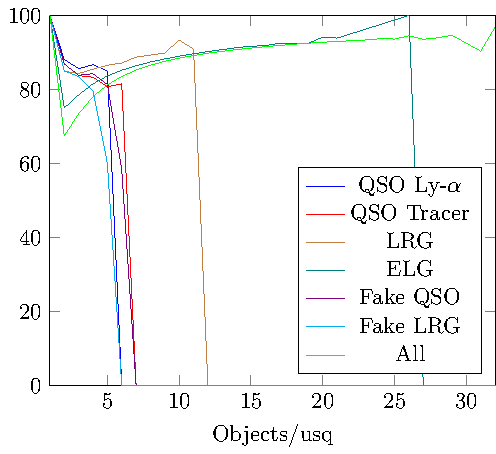
\includegraphics[scale=1]{figs/graph/seendens.pdf}
	\caption{\% of observed galaxies as a function of objects density}\label{seendens}
\end{center}\end{figure}


\subsection{Results on \lya particularly}
Figure \ref{histastf} gives the histogram of proportion of assigned \lya and the number of observations as a function of available tile-fibers.

\begin{figure}[H]\begin{center}
	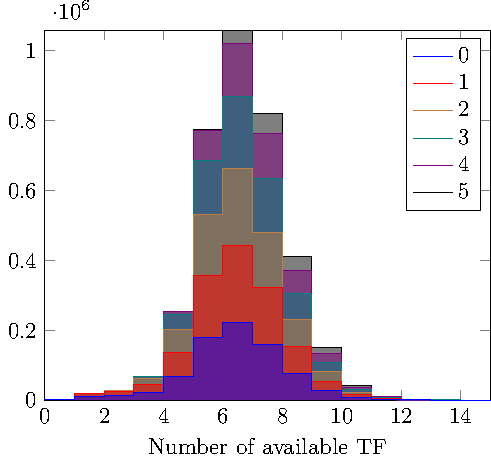
\includegraphics[scale=1]{figs/graph/obsly.pdf}
	\caption{\# of QSO \lya (with their number of observation) as a function of available tile-fibers}\label{histastf}
\end{center}\end{figure}

\begin{figure}[H]\begin{center}
	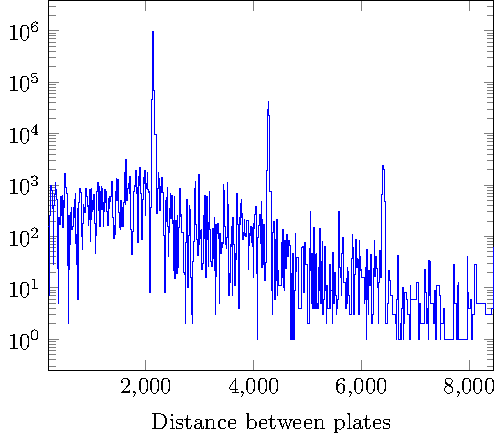
\includegraphics[scale=1]{figs/graph/dist2ly.pdf}
	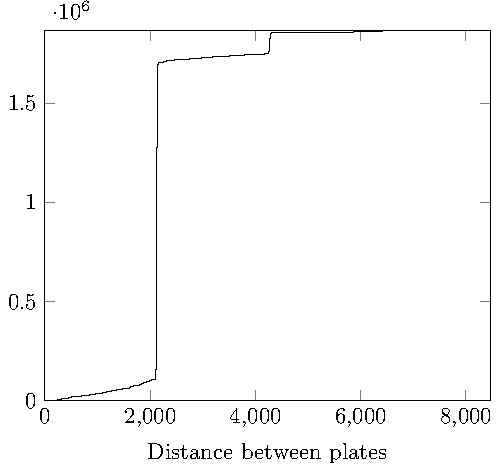
\includegraphics[scale=1]{figs/graph/dist2lyint.pdf}\hfill
	\caption{Histogram of distances (in number of plates) between two consecutive observed QSO \lya and integral}
\end{center}\end{figure}

\subsection{Study on evolution over time}

\begin{figure}[H]\begin{center}
	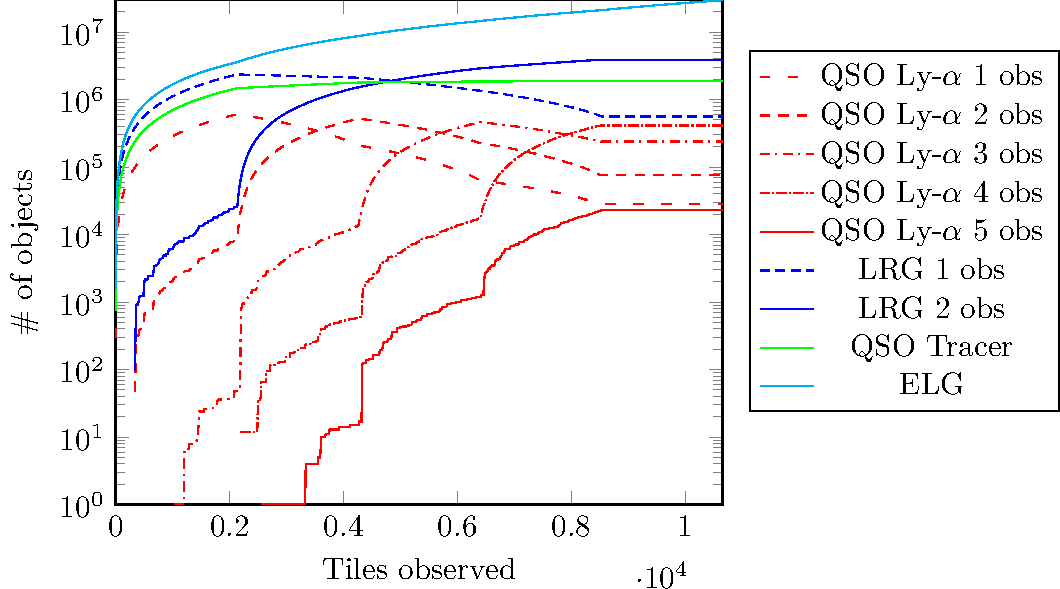
\includegraphics[scale=1]{figs/graph/time2.pdf}
	\caption{Observed galaxy kind as a function of time (plates seen)}
\end{center}\end{figure}

\subsection{Choice by density}
The assignment could include the idea well described in $[1]$ which consists in, when you have the choice of several fibers to observe an object, you choose the one which has the least density of (weighted) remaining available objects in reach. This way, "busy" fibers are more available. Of course, it will introduce a bias in the survey, and since it doesn't improve results (it's likely because redistribution/improvement functions already make this optimization) we can avoid it. An illustration taken from $[1]$ is in Figure \ref{act}.

\begin{figure}[H]\begin{center}
	\includegraphics[scale=0.15]{figs/act.eps}
	\caption{Choice by density : A is chosen to observe 1}\label{act}
\end{center}\end{figure}

\subsection{Tiling strategy}
The tiling strategy is important and should separate overlapping tiles for more than "Analysis". This way, the assignment can be updated in order to avoid observing twice the same object. The results are then improved in a non negligible rate. Fiber assignment results may help to choose the best strategy.


\section{Collision problem}
Fiber geometry can be found at \href{https://desi.lbl.gov/DocDB/cgi-bin/private/ShowDocument?docid=899}{this address}, which is a work of Joe Silber. The exact geometry as built in our program can be seen on Figure \ref{onefib}, which consists in two circles and several segments. The black dot point is the center of the positioner, and other ones are objects in reach.

\begin{figure}[H]\begin{center}
	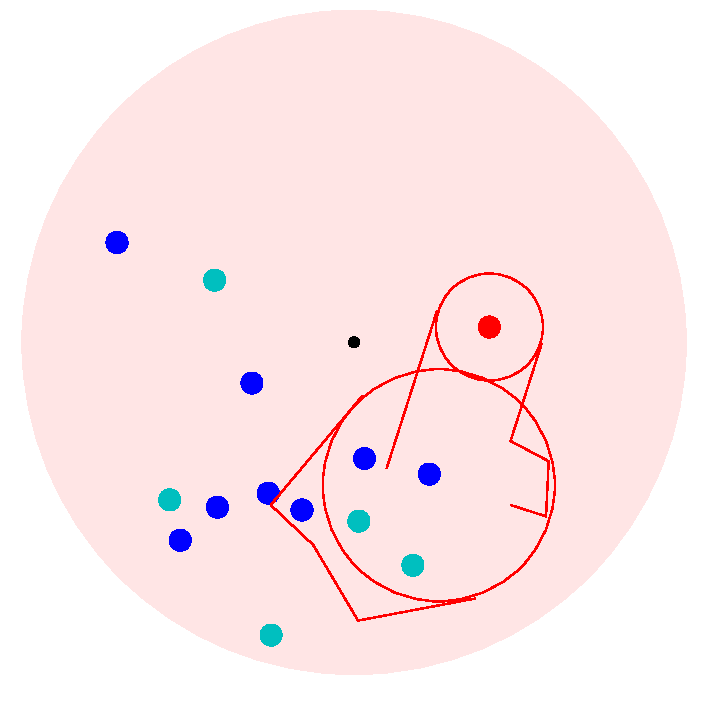
\includegraphics[scale=0.7]{figs/one_fib.pdf}
	\caption{Geometry of a fiber positioner, with fiber holder and central body oriented}\label{onefib}
\end{center}\end{figure}

In the features file the "Exact" boolean indicates whether we choose the exact geometry of the fiber positioners. If not, collisions are computed with only circles at the position of the fiber holder, of radius $AvCollide$, which we calibrate such that we get the same collision rate than with the exact geometry ($\sim$ 10.8\% of fibers collide). If the exact geometry is on, the modules collision.h and collision.cpp are used to check. They then build sets of circles or segments, and check collisions between those belonging to the first fiber positioner to the ones belonging to the second one.
Computationnally cheap methods were absolutely necessary and used for segment-segment and circle-segment checking, because checking functions are called a lot of time, and optimization of those methods lead to considerably decrease total computation time. That is why we use circle and segments, not only segments : creating an arc with segments needs a lot of them, but only one circle.

Figure \ref{coldist} is the histogram of distances between two galaxies, in a collision case, and its integral.

\begin{figure}[H]\begin{center}
	\includegraphics[scale=1]{figs/graph/coldist.pdf}
	\includegraphics[scale=1]{figs/graph/coldistint.pdf}
	\caption{Histogram of distances between galaxies in collision case, and integral}\label{coldist}
\end{center}\end{figure}

$[2]$ is an article about the problem of reaching final position for the positioner without colliding a neighboring one.

\section{Tile ploting}
The function pyplotTile builds a tile.py file, which can be executed manually with {\tt python tile.py} to create the pdf plot.
Only objects that would need at least one remaining observation are projected on the plate and ploted. The function has to be called just before real observation time, otherwise, if it is called at the end for example, information on number of observations of an object would be the one that we have at the end, and not on the way.

A grey circle is ploted when there is an unassigned fiber at some place, not to mix up with fiducials (totally white), places where there is physically no fiber.
Watching at a dozen of tile plots, one can convince oneself that the assignment is very close to the optimum.

\begin{figure}[H]
\hspace*{-1.5cm}
    \includegraphics[scale=1.75]{python/rep-1000.pdf}
	\caption{Tile 1000}
\end{figure}

\section{Other functions}
In the library, functions are written to put data into .dat files, which can be compiled by the Latex module Tikz to create figures like histograms present here.

There is a function of verification which check several features of the assignment to know if it is sane (no collision, regular mapping, etc...).

\section{Effect on correlation function}
One of the difficulties is that we have not to bring experimental bias the way we do the assignment. The fact that a lot of rules are used in the assignment makes it more likely that a bias is created.
We can do a study, comparing correlation functions given with this fiber assignment and ones with all galaxies.


\section{Mathematical optimum}
Have we reached the optimum ? We have to master, understand, results we get from mathematical computations.

Imagine a portion S of the sky of the size the reacheable area by a single fiber. Let i be the indice for different kinds (\lya, fake QSO, ... except SS or SF). Let $\lambda_{i}$ be the densities of the kinds of objects in S. Let N be the indice for the portions of sky with exactly N objects (when we take an area of size S). Let $f_{N}$ be the fraction of the sky which density corresponds to N. Let $poisson(x,n) = \frac{x^{n}e^{-x}}{n\text{!}}$ be the Poisson distribution. Then, for a given ELG in S, named e, the probability to be observed is :

	\begin{equation}
\begin{split} 
	p(\text{observe e}) =& \sum\limits_{1 \le N \le 10} f_{N} \sum\limits_{0 \le A \le N-1\text{ and }1 \le B \le \infty} p(\text{\tiny A objects having priority over an ELG}) \cdot p(\text{\tiny B ELG and e is chosen among the N-A firsts})\\
	=& \sum\limits_{1 \le N \le 10} f_{N} \sum\limits_{0 \le A \le N-1\text{ and }1 \le B \le \infty} p(A) \cdot p(\text{\tiny B ELG}) \cdot p(\text{\tiny e is chosen among the N-A firsts})\\
	=& \sum\limits_{1 \le N \le 10} f_{N} \sum\limits_{0 \le A \le N-1} \sum\limits_{1 \le B \le \infty} p(A) \cdot \frac{\lambda_{ELG}^{B}e^{-\lambda_{ELG}}}{B\text{!}} \cdot \frac{N-A}{B}\\
	=& I\cdot\sum\limits_{1 \le N \le 10} f_{N} \sum\limits_{0 \le A \le N-1} p(A) (N-A)
\end{split} 
	\end{equation}

	where $I = e^{-\lambda_{ELG}} \int\limits_{0}^{\lambda_{ELG}} \frac{e^{\lambda}-1}{\lambda} d\lambda$ 
	
	Also we define the set L of objects with priority against ELG, which are \lya, fake QSO, QSO target, LRG and fake LRG. Then, for $i \in L$ :
	
	$p(A) = \sum\limits_{n_{i} st \sum\limits_{i} goal(i)n_{i} = A} \prod\limits_{i} poisson(\lambda_{i},n_{i})$

	One use the same method to compute theoretical percentage of observed QSO and LRG.

\section{Possible improvements}
One could try to search for an "orthogonal" (of the 3 other ones) improvement function.

Nevertheless, it is likely that we are almost at the global optimum.

Other ideas from $[1]$.


\bibliographystyle{plain}
%\bibliography{papers}{}

  \begin{thebibliography}{1}

  \bibitem{fa} Morales {\em Fiber assignment in next-generation wide-field spectrographs}  2012.

  \bibitem{collision} Makarem {\em Collision avoidance in next-generation fiber positioner robotic systems for large survey spectrographs}  2014.

  \end{thebibliography}

\end{document}
